\documentclass[margin=3pt,
  convert,
  convert={
    outext=.png,
    command=\unexpanded{
      pdftocairo -r 300 -png \infile % 将生成的pdf文件转换为png图像
    }
  }
  ]{standalone}

\usepackage{tikz}
\usetikzlibrary{intersections, calc}

% 求两个路径交点
% #1 第1路径名称
% #2 第2路径名称
% #3 交点名称,同时定义了一个全局宏\InterNb记录了交点总数
\newcommand{\intersec}[3]{%
  \path[name intersections={of=#1 and #2, by=#3, sort by=#1,total=\t}]
  \pgfextra{\xdef\internb{\t}};
}

% 过指定点到曲线的垂线
% #1 路径名称
% #2 路径上指定点坐标
% #3 交点坐标
\newcommand{\insecvline}[3]{
  % 过#2点的垂线
  \path[name path = v](#2|-current bounding box.south) -- (#2|-current bounding box.north);  
   % 求路径#1与路径v的交战,并记为#3
  \intersec{#1}{v}{#3}
}

\begin{document}
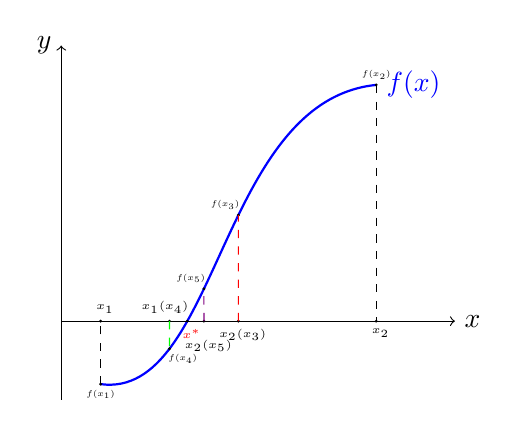
\begin{tikzpicture}[
  domain=1.5:4.1,
  samples=101,
  ]
  % 绘制命名曲线
  \draw[blue,thick, name path=graph](0.5,-0.8) coordinate (fx1) .. controls (2.0,-1) and
  (2,2.8) .. (4, 3) coordinate (fx2) node[right] {$f(x)$};
  % 绘制x轴和y轴
  \draw[->, name path=x] (0,0) -- (5,0) node[right] {$x$};
  \draw[->] (0,-1.0) -- (0,3.5) node[left] {$y$};

  % 绘制根的真值点
  \intersec{graph}{x}{x0}
  \fill[fill=black](x0) circle[radius = 0.02cm] node[red, scale = 0.8,
  below, shift={(2pt, 0pt)}, font=\tiny]{$x^*$};
  
  % 初始点坐标定义
  \coordinate (x1) at (0.5, 0);
  \coordinate (x2) at (4.0, 0); 

  % 迭代初值
  \fill[fill=black](x1) circle[radius = 0.02cm] node[black, scale = 0.8,
  above, shift={(2pt, 0pt)}, font=\tiny]{$x_{1}$};
  \fill[fill=black](x2) circle[radius = 0.02cm] node[black, scale = 0.8,
  below, shift={(2pt, 0pt)}, font=\tiny]{$x_{2}$};
  % 初值垂线及函数值标记
  \draw[black, dashed] (fx1) -- (x1);
  \draw[black, dashed] (fx2) -- (x2);
  \fill[fill=black](fx1) circle[radius = 0.02cm] node[black, scale =
  0.6, below, shift={(0pt, 0pt)}, font=\tiny]{$f(x_{1})$};
  \fill[fill=black](fx2) circle[radius = 0.02cm] node[black, scale =
  0.6, above, shift={(0pt, 0pt)}, font=\tiny]{$f(x_{2})$};

  % 迭代循环
  % \X---迭代编号
  % \sel---迭代后x1,x2中选中的编号(1或2)
  % \xvpos---x轴标记位置(above,below,left,right)
  % \fvpos---f(x)值标记位置(above,below,left,right)
  % \xvoff---x轴标记的垂直偏移量(需要指明单位pt)
  % \clr---本次迭代垂线着色
  \foreach \X/\sel/\xvpos/\fvpos/\xvoff/\clr in
  {
    3/2/below/above/0pt/red,
    4/1/above/below/0pt/green,
    5/2/below/above/-5pt/violet}
  {
    % 求出x1和x2的中点坐标
    \coordinate (bx) at ($(x1)!0.5!(x2)$);
    % 求过bx的垂线与曲线交点坐标
    \insecvline{graph}{bx}{fx}
    % 绘制x轴坐标点和对应函数值点
    \ifodd\sel% 迭代后选择x1
      \fill[fill=black](bx) circle[radius = 0.02cm] node[black, scale = 0.8,
      \xvpos, shift={(-2pt, \xvoff)}, font=\tiny]{$x_{\sel}(x_{\X})$};
      \fill[fill=black](fx) circle[radius = 0.02cm] node[black, scale = 0.6,
      \fvpos, shift={(8pt, 0pt)}, font=\tiny]{$f(x_{\X})$};
    \else% 迭代后选择x2
      \fill[fill=black](bx) circle[radius = 0.02cm] node[black, scale = 0.8,
      \xvpos, shift={(2pt, \xvoff)}, font=\tiny]{$x_{\sel}(x_{\X})$};
      \fill[fill=black](fx) circle[radius = 0.02cm] node[black, scale = 0.6,
      \fvpos, shift={(-8pt, 0pt)}, font=\tiny]{$f(x_{\X})$};
    \fi
    % 绘制x轴坐标点和对应函数值点间的垂线  
    \draw[\clr, dashed] (bx)--(fx);   
  
    % 准备下一次迭代
    \coordinate (x\sel) at (bx);
  }
\end{tikzpicture}
\end{document}

%%% Local Variables:
%%% mode: latex
%%% TeX-master: t
%%% End:
